\chapter{RC Circuits} \label{chap:RC}
\section{RC Circuits}
An RC circuit is an electrical circuit consisting of resistors and capacitors. In its simplest form, it is composed of one of each. In that case, a charged capacitor placed in series with a resistor will discharge back through the resistor \cite[p~21]{artof}. 

\begin{figure}[H]
 \begin{center}
\begin{circuitikz}[american voltages]
\draw (0,0)
to[sqV, sqV=$v_{input}$] (0,2)
to (6,2)
to[short, -] (4,2)
to[C=$C$] (4,0)
to (6,0)
to (4,0)
to [resistor, R=$R$] (0,0);
\draw [>=latex', <->] (6,1.75) -- node[anchor=west] {$v_{C}(t)$} (6,0.25);
\end{circuitikz}
\end{center}
 \caption{A simple RC circuit with a voltage input, a capacitor and a resistor}
\end{figure}
\subsection{Transient Analysis}
\label{sec371}
To find out how the voltage of a capacitor changes over time when it is charged and discharged, transient analysis is used.
\\
\\
\textbf{Discharging of a Capacitor}\\
In subsection \ref{Klaws}, KCL states that the sum of the currents in a node is equal to zero. In the case of an RC circuit, the law can be written as the following equation:
\begin{align}
i_{C}+i_{R}&=0 \nonumber \\
i_{C}&= -i_{R}, \label{Ic-Ir}
\end{align}
where $i_C$ is the current through the capacitor, and $i_R$ is the current across the resistor. From \eqref{iC} the current through the capacitor is:
\begin{align}
	i_C(t) = C\frac{dv_C(t)}{dt}\label{iC=Cdv}
\end{align}
The equation for the current across the resistor \eqref{Ohm}, can be rewritten as:
\begin{align}
	i_R(t) = \frac{v_R(t)}{R}\label{iR=vR}
\end{align}
Inserting the definitions in \eqref{iC=Cdv} and \eqref{iR=vR}, into \eqref{Ic-Ir} gives:
\begin{align*}
	C\frac{dv_C(t)}{dt} = \frac{-v_R(t)}{R}
\end{align*}
Both sides are divided by $C$:
\begin{align}
	\frac{dv_C(t)}{dt} =-v_R(t) \frac{1}{RC}
	\label{eq:dvC(t)}
\end{align}
From KVL, it can be derived that:
\begin{align}
	v_R(t) - v_C(t) = 0\nonumber\\
	v_R(t) = v_C(t) \label{vR(t)}
\end{align}
\eqref{vR(t)} is inserted into \eqref{eq:dvC(t)}:
\begin{align*}
	\dfrac{dv_C(t)}{dt} &= \dfrac{-1}{RC}v_C(t)
\end{align*}
The equation is now in the same form as \eqref{SDEG}, and can be solved as following:
\begin{align}
\int \dfrac{1}{v_C(t)}dv_C(t) =& \dfrac{-1}{RC} \int dt\nonumber \\
\ln(v_C(t)) =& \dfrac{-t}{RC} + A \nonumber\\
v_C(t) =& e^{\frac{-t}{RC}}e^{A}\label{V_eA}
\end{align}
Since $A$ is the constant of integration, $e^A$ is a constant aswell.
\\
By definition, the starting voltage of the capacitor is given by $v_C(t=0)=v_0$:
 \begin{align*}
	v_C(0) &= e^{\frac{0}{RC}}e^A\\
	v_C(0) &= e^A
 \end{align*}
Therefore $e^A = v_0$, and this can be inserted into \eqref{V_eA}:
\begin{align}
\label{V_down}
\Aboxed{
 v_C(t) = v_0e^{\frac{-t}{RC}}
 }
\end{align}
The function in \eqref{V_down} describes how the voltage decreases over time, when the capacitor is discharged.
\\
\\
\textbf{Charging of a Capacitor}\\
In subsection \ref{Klaws}, KVL states that the sum of the voltages over a loop must be equal to zero. 
\\
In an RC circuit with a battery, the algebraic sum can be written as:
\begin{align}
v_{input}(t)-v_R(t)-v_C(t) =& 0 \nonumber \\
v_{input}(t) =& v_R(t)+v_C(t), \label{V_B}
\end{align}
where $v_{input}(t)$ is the voltage of the battery, $v_R(t)$ is the voltage of the resistor, and $v_C(t)$ is the voltage across the capacitor. $v_R(t)$ and $v_C(t)$ have negative signs, since their elements create a negative potential difference when charge passes through them.
\\
From \eqref{Ohm}, the voltage drop across the resistor can be expressed as $v_R(t)=I_R R$. From \eqref{QCV} the voltage drop across the capacitor can be expressed as $v_C(t)=\dfrac{q_C (t)}{C}$. This is inserted into \eqref{V_B}:
\begin{align}
v_{input}(t) =& I_R R + \dfrac{q_C (t)}{C} \label{Vb=IR}
\end{align}
As stated in \eqref{I=dq/dt}, current is defined as $I =\dfrac{dq}{dt}$, and this is inserted into \eqref{Vb=IR}.
 \begin{align*}
 	v_{input}(t) &= \frac{dq_R(t)}{dt} R + \frac{q_C (t)}{C}
 \end{align*}
Both sides are divided by $R$:
\begin{align}
\dfrac{v_{input}(t)}{R} &= \dfrac{dq_R(t)}{dt} + \dfrac{1}{RC}q_C(t)\label{Vb/R} 
\end{align}
This is now a linear differential equation of the first order in the form of \eqref{FODE_form}:
\begin{align*}
\dfrac{dy}{dx}+h(x)y=g(x)
\end{align*}
If the conditions for the general solution for a linear differential equation of the first order are fulfilled, \eqref{Vb/R} can be solved like in \Cref{linethe}:
\begin{align*}
y&=e^{-H(x)}\left(\int e^{H(x)}g(x)dx+C\right)
\end{align*}
The terms in \eqref{Vb/R} represent these terms in the general solution:
\begin{align*}
y &= q_C(t)
\\
h(x) &= \dfrac{1}{RC}
\\
H(x) &= \int \dfrac{1}{RC}dt=\dfrac{t}{RC}
\\
g(x) &= \dfrac{v_{input}(t)}{R}
\\
\dfrac{dy}{dx} &= \dfrac{dq_R(t)}{dt}
\end{align*}
Then the general solution for \eqref{Vb/R} is:
\begin{align*}
q_C(t) &= e^{\frac{-t}{RC}}\int_{0}^{t}e^{\frac{t}{RC}}\dfrac{v_{input}(t)}{R}dt
\end{align*}
The constant is put outside the integral:
\begin{align}
q_C(t) &= e^{\frac{-t}{RC}}\dfrac{v_{input}(t)}{R}\int_{0}^{t}e^{\frac{t}{RC}}dt \label{Q_1}
\end{align}
The integral is now solved by substitution. First $u$ and $\dfrac{du}{dt}$ are defined:
\begin{align*}
u &= \dfrac{t}{RC}
\\
\dfrac{du}{dt}&=\dfrac{1}{RC}
\\
dt &=RC du
\end{align*} 
By inserting these definitions into \eqref{Q_1} the equation looks like this:
\begin{align*}
q_C(t) &= e^{\frac{-t}{RC}}\dfrac{v_{input}(t)}{R}\int_{0}^{\frac{t}{RC}}RCe^u du
\\
q_C(t) &= e^{\frac{-t}{RC}}\cdot v_{input}(t)\cdot C\cdot \left[e^u\right]_{0}^{\frac{t}{RC}}
\\
q_C(t) &= v_{input}(t) \cdot C\cdot e^{\frac{-t}{RC}}\cdot\left(e^{\frac{t}{RC}}-1\right)
\\
q_C(t) &= v_{input}(t) \cdot C \cdot \left(1-e^{\frac{-t}{RC}}\right)
\end{align*} 
The voltage of a capacitor is given as $v_C(t)=\dfrac{q_C(t)}{C}$. By dividing the equation above with $C$, the function for charging a capacitor is found.
\begin{align}
\label{V_up}
\Aboxed{
v_C(t)=v_{input}(t)\left(1-e^{\frac{-t}{RC}}\right)
}
\end{align}
\section{RC circuit experiment} \label{c: RC_exp}
In the following section an RC circuit experiment has been made. Data from an RC circuit will be compared to values from a mathematical model.

\subsection{Theoretical Values}
The resistor and capacitor in the experiment, had the following values:
\begin{align*}
 R =& 4770\Omega \\
 C =& 97.61nF
\end{align*}
The circuit was set up as follows:
\begin{figure}[H]
	\begin{center}
\begin{circuitikz}[american voltages]
\draw
to[sqV, sqV=$1 V$] (0,2)
to[resistor, R=$4770 \Omega$] (4.5,2)

[short](3,2) to [short] (5,2)

to [short, C=$97.61 nF$] (5,0)
(0,0) to [short, -] (5,0)

(0,1) to [short, -] (0,2);
\end{circuitikz}
\end{center}
	\caption{A circuit with a resistor(4770$\Omega$) and a capacitor(97.61nF)}
\end{figure}
\noindent The time constant $\tau$, is defined as $\tau = RC$. In this case $\tau$ is:
\begin{align*}
	\tau = 4.77 k\Omega \cdot 97.61 nF &= 46.56 \cdot 10^{-5} s \\
\end{align*}
Furthermore, the charging and discharging of the capacitor can then be put in a table. Since the formula $v_{charge}(t)=v_{input}(t)(1-e^{\frac{-t}{RC}})$ contains $e^{\frac{-t}{RC}}$, the table values can be calculated for different $\tau$ values. $v_{charge}(t)$ can be calculated as follows for $\tau = 2$: 
\begin{align*}
v_{charge}(t)=v_{input}(t) \cdot \left(1-e^{\left(\frac{\left(-2 \cdot \left(46.56 \cdot 10^{-5} \right)\right)}{46.56 \cdot 10^{-5}}\right)} \right) = v_{input}(t)(0.865)
\end{align*}
Here $86.5\%$ is the table value for two $\tau$. The formula for $v_{discharge}(t)$ was derived in section \ref{sec371} as: $v_{C}(t)=v_{0} \left(e^{\frac{-t}{\tau}} \right)$. $v_{discharge}$ for $\tau = 2$ can be calculated as:
\begin{align*}
v_{discharge}(t)=v_{0} \cdot \left(e^{\left(\frac{\left(-2 \cdot \left(46.56 \cdot 10^{-5} \right)\right)}{46.56 \cdot 10^{-5}}\right)} \right) = v_{0}(0.135)
\end{align*}
The table value for $\tau = 2$ is therefore $13.5 \%$ for $v_{discharging}(t)$. \\
Hereby a table can be created for $v_{charge}(t)$ and $v_{discharge}(t)$: \\
\begin{table}[H]
\center
\begin{tabular}{|l|l|l|}
\hline
$\tau$ & $v_{charge}(t)$ & $v_{discharge}(t)$ \\ \hline
1      & 63.2\%       & 36.8\%         \\ \hline
2      & 86.5\%       & 13.5\%         \\ \hline
3      & 95.0\%       & 5.0\%          \\ \hline
4      & 98.2\%       & 1.8\%          \\ \hline
5      & 99.3\%       & 0.7\%          \\ \hline
\end{tabular}
\caption{$\tau$ charge and discharge percentages}
\end{table}
\noindent Generally, the capacitor is considered fully charged, or discharged, at $5\tau$. \\
The time it takes for the capacitor to be fully charged, or discharged, is in this case:
\begin{align*}
5\tau &= 5 \cdot 46.56 \cdot 10^{-5} s \\
&= 2.33 ms
\end{align*}

\subsection{Test Values Comparison}
\begin{figure}[H]
	\center
		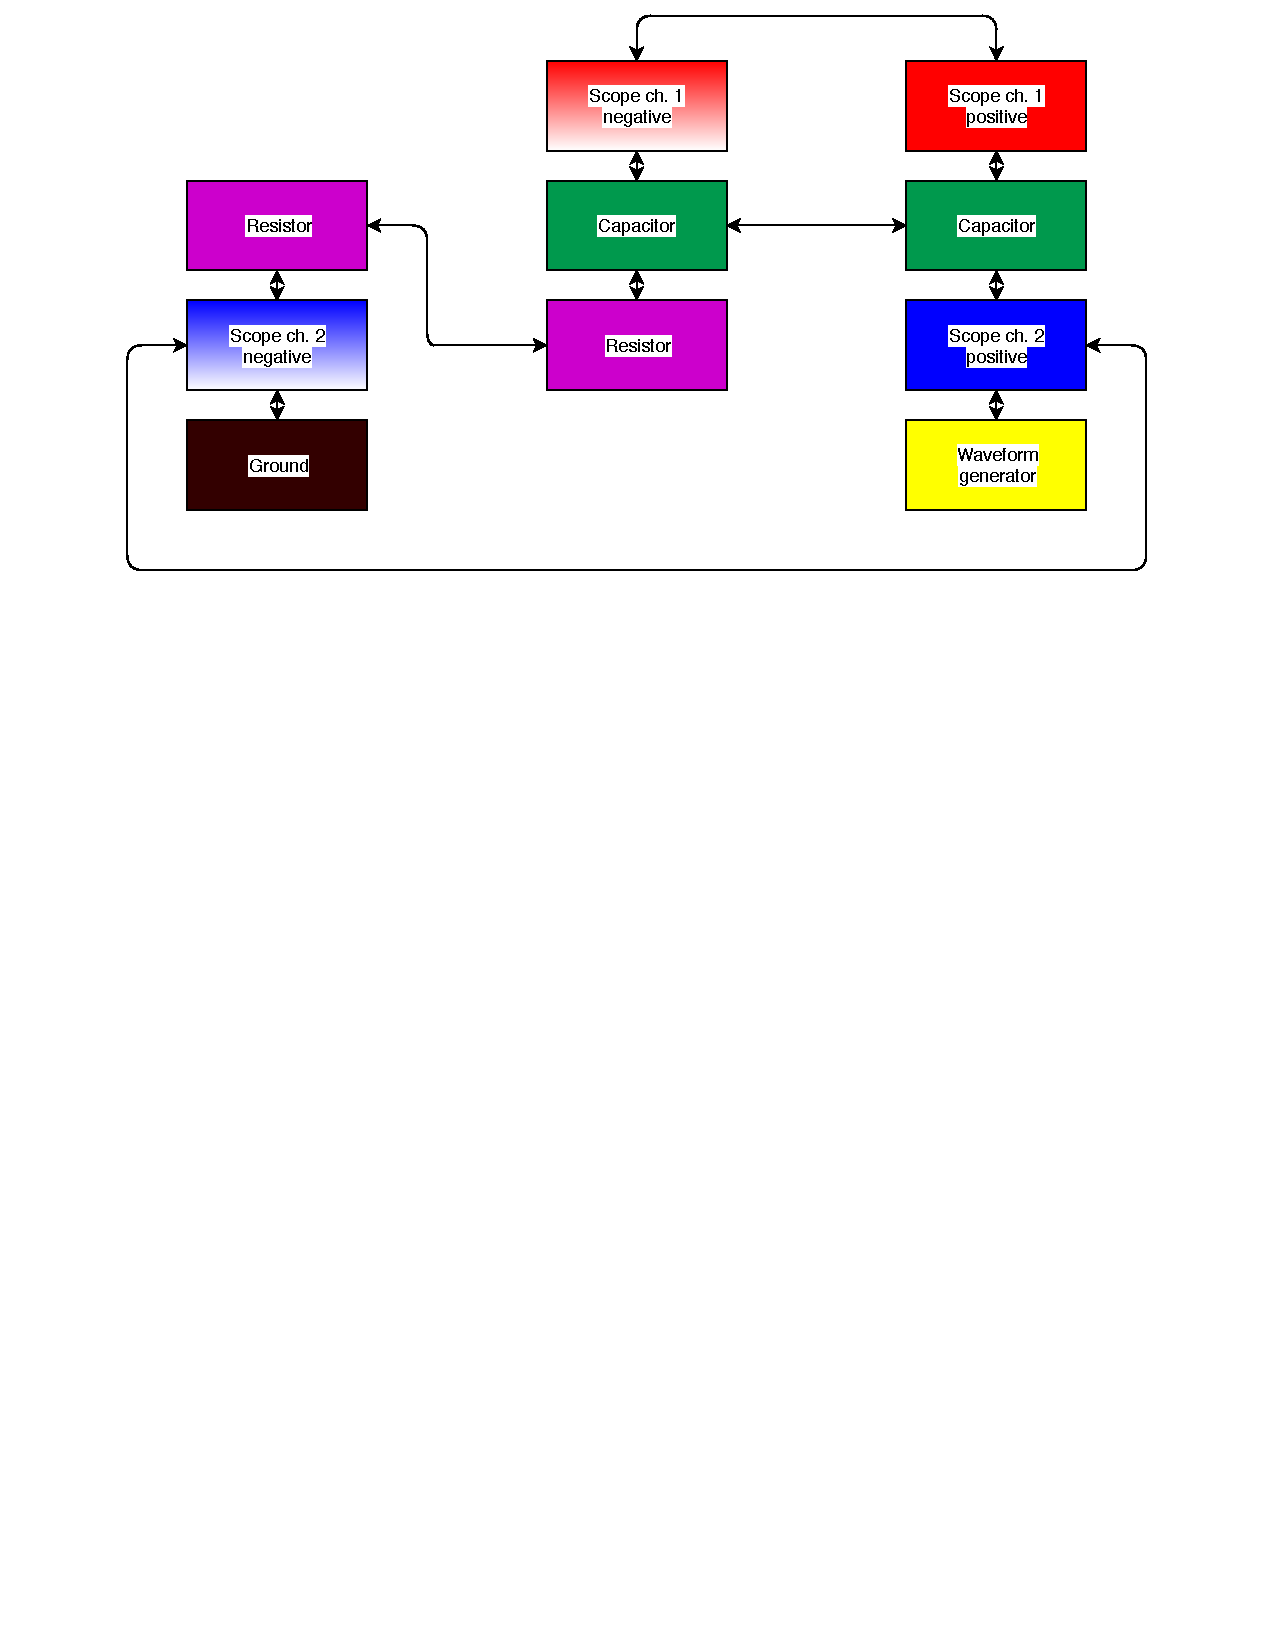
\includegraphics[clip, trim=0cm 18cm 0cm 0cm, scale=0.6]{fig/img/test_circuit_1}
	\caption{Setup of the RC circuit used in the experiment}
	\label{rc_flow}
\end{figure}
% Vær OBS på farvebeskrivelser af ledninger
This section uses the Analog Discovery 2 for setting up an RC circuit. The first step of the set-up is inserting a positive waveform generator (yellow) and a positive scope (blue) showing the waveforms. The waveform generator uses an AC step voltage. The current then passes through a resistor ($4.77 k\Omega$) and a capacitor ($97.61 nF$). Another scope is inserted to measure the charging and discharging of the capacitor. First, the current passes through a positive scope (orange), then the capacitor, and back through a negative scope (orange/white). Hypothetically, if the two scopes were switched, it would be measuring the inverse charging and discharging. Lastly, the current passes through a negative scope (blue/white) and into a negative waveform generator (yellow/white). Hereby, the circuit illustrated in figure \ref{rc_flow} is created with the same values as in the previous section. \\ \\
To get the test values compatible with the theoretical values, the frequency input has to be calculated as the hertz needed for the capacitor to charge and discharge. Therefore, the wave generator has to produce $214.6 Hz$  ($(2 \cdot 2.33 ms)^{-1} = 214.6 Hz$). \\
The data from the theoretical values and the test results can now be compared using python:
\begin{figure}[H]
\center
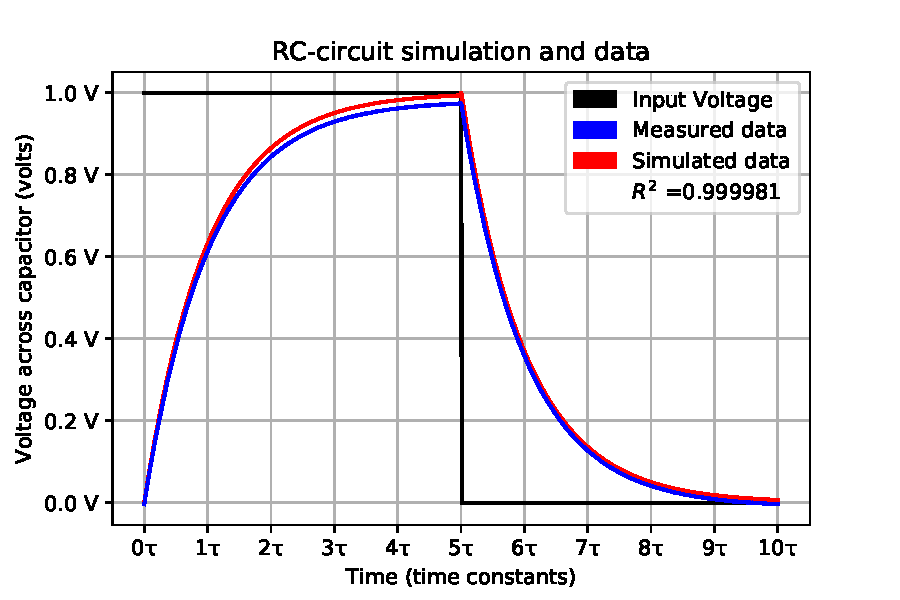
\includegraphics[scale=0.6]{fig/img/eks_1}
\caption{The measured and simulated data for the charge and discharge of a capacitor}
\label{fig:Cap}
\end{figure}
\noindent As shown on the graph, the test results are very close to the calculated theoretical values. the coefficient of determination, $R^2$, is almost equal to 1, which means that the two plots are almost identical.

\subsection{Uncertainty}
Values from experiments rarely agree completely with the theoretical values. The coefficient of determination, $R^2$, is an expression for the uncertainty between two plots. As seen in figure \ref{fig:Cap}, $R^2$ is very close to $1$, which means there is some uncertainty. If the measured data was exactly the same as the simulated data, $R^2$ would be $1$. This uncertainty can be caused by a few different reasons. The components in the circuit might have a bit of resistance, and the capacitors integrity might not be perfect, because of usage or time, and there might be a small energy loss when running the experiment. 